\documentclass[times, utf8, seminar, numeric]{fer}
\usepackage{booktabs}

\begin{document}

% TODO: Navedite naslov rada.
\title{Trojanski napadi na modele za semantičku segmentaciju}

% TODO: Navedite vaše ime i prezime.
\author{Dominik Jambrović}

% TODO: Navedite ime i prezime mentora.
\voditelj{prof.\ dr.\ sc.\ Siniša Šegvić}

\maketitle

\tableofcontents

\chapter{Uvod}

U današnje vrijeme, duboki modeli primjenjuju se u brojnim aspektima svakodnevnog života.\ Pritom se pažnja primarno posvećuje performansama i konzistentnosti modela.\
Nažalost, sigurnosni aspekt često je zapostavljen.\ Kada govorimo o sigurnosti dubokih modela, važno je prvo identificirati moguće prijetnje.\ 
Neke od najčešćih su neprijateljski primjeri~\cite{goodfellow2014explaining} i zatrovani podatci~\cite{chen2017targeted}.\
  
Područje računalnog vida obuhvaća brojne zadatke.\ Jedan od najčešće rješavanih zadataka je klasifikacija – model na ulazu dobiva primjer te na izlazu treba dati jednu oznaku koja predstavlja razred u koji je ulaz svrstan.\ 
Brojna istraživanja fokusirala su se na primjenu napada na ovakve modele, kao i na potencijalne obrane.\ Naravno, ne možemo rješavati sve probleme iz stvarnog života koristeći obične klasifikatore.\ 
Za neke zadatke (npr. „vid“ autonomnih vozila), potrebni su nam modeli koji će svaki piksel ulaza zasebno klasificirati u određeni razred.\ Ovaj zadatak zovemo semantička segmentacija~\cite{garcia2017review}.\
Model na ulazu dobiva sliku, a na izlazu treba dati novu sliku (segmentaciju) gdje je svakom pikselu iz ulaza dodijeljena oznaka pripadnog razreda.\ Cilj ovog rada je reprodukcija napada na odabrani model za semantičku segmentaciju po uzoru na rad~\cite{li2021hidden}.

\chapter{Semantička segmentacija}

\section{Arhitektura SwiftNet}

Sve eksperimente provodili smo na arhitekturi Single-Scale SwiftNet~\cite{orvsic2021efficient}.\ Ovaj model sastoji se od kodera koji provodi poduzorkovanje, sloja prostornog piramidalnog sažimanja i dekodera koji provodi naduzorkovanje.\ 
Pritom se za okosnicu kodera koristi model ResNet18~\cite{he2016deep} prednaučen na skupu ImageNet~\cite{deng2009imagenet}.\ Slojevi kodera i dekodera povezani su lateralnim vezama (ljestvičasta arhitektura).\

\begin{figure}[htb]
    \centering
    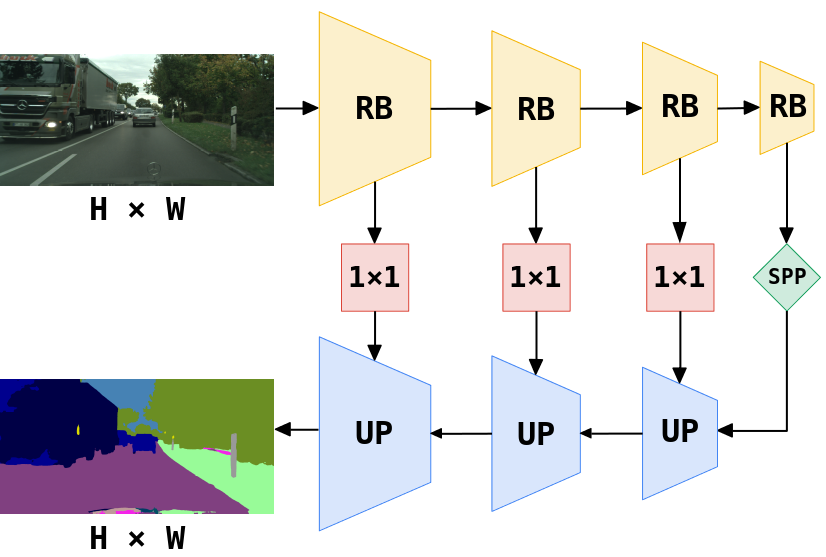
\includegraphics[scale=0.425]{./Slike/swiftnet.png}
    \caption{Arhitektura Single-Scale SwiftNet. Preuzeto iz~\cite{orvsic2021efficient}.}
    \label{fig:swiftnet}
\end{figure}

\chapter{Napadi na modele strojnog učenja}

\section{Neprijateljski primjeri}

Neprijateljski primjeri većinom su slike na koje je nadodan šum (najčešće konstruiran gradijentnim metodama).\ Cilj ove vrste napada je izmijeniti odluku već naučenog modela i time izbjeći ispravnu klasifikaciju.

\section{Zatrovani podatci}

Zatrovani podatci najčešće su parovi izmijenjenih slika i proizvoljno odabranih oznaka.\ Pritom se na originalne slike većinom dodaje okidač (npr. nekoliko bijelih piksela u kutu slike).\ Cilj ove vrste napada je da se model nauči na zatrovanim podatcima te da napadač time ugradi stražnja vrata u model.

\chapter{Skup podataka ADE20k}

Skup ADE20k~\cite{zhou2019semantic} sastoji se od otprilike 25 000 označenih slika iz stvarnog života. Podijeljen je na 20 210 slika u skupu za učenje, 2000 slika u skupu za validaciju te 3000 slika u skupu za ispitivanje.\ 
Svaki piksel može pripadati jednom od ukupno 150 razreda.\ Ulazne slike, kao i pripadne segmentacije, varirajućih su dimenzija.
  
\begin{figure}[htb]
    \centering
    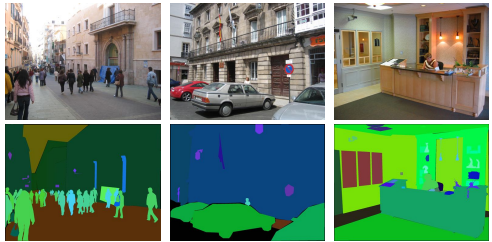
\includegraphics[scale=1]{./Slike/ade20k.png}
    \caption{Primjeri slika i oznaka iz skupa ADE20k. Preuzeto iz~\cite{zhou2019semantic}.}
    \label{fig:ade20k}
\end{figure}
\chapter{Eksperimenti}

\section{Postavke eksperimenata}

Eksperimente smo provodili učenjem modela na prirodnom skupu podataka, kao i na nekolicini zatrovanih skupova podataka.\ Pritom su za stvaranje zatrovanih skupova podataka korišteni razni okidači, kao i razne izmjene segmentacijskih oznaka.\ 
Okidače općenito možemo podijeliti na nesemantičke i semantičke.\ Nesemantički okidači podrazumijevaju izmjenu ulazne slike (npr. dodavanje nekoliko bijelih piksela u kut slike).\ S druge strane, semantički okidači ne mijenjaju ulaznu sliku.\ 
Umjesto toga, kao zatrovani primjeri se uzimaju ulazne slike koje sadrže piksele koji pripadaju određenom razredu (npr. slike s barem jednim pikselom iz razreda Wall).
  
Kao nesemantičke okidače, koristili smo crnu liniju širine 8 piksela dodanu na vrh ulazne slike, kao  i crni okvir širine 8 piksela dodan na rub ulazne slike.\ Kao semantičke okidače, birali smo slike koje sadrže barem jedan piksel iz razreda Grass ili iz razreda Wall.\ 
Kada govorimo o izvedbi trovanja, radimo podjelu na napade na razini slike odnosno primjerka.\ Za napad na razini slike, nasumično smo odabrali oznaku koja sadrži barem jedan piksel iz razreda Road.\ Svakom zatrovanom primjeru dodijelili smo oznaku odabrane slike, pritom provodeći prikladno skaliranje zbog varirajućih dimenzija primjera.\ 
Kod napada na razini primjerka, segmentaciju zatrovanih primjera izmijenili smo tako da pikseli koji pripadaju razredu Person sada pripadaju razredu Palm.
  
Svi modeli učeni su 200 epoha, a pri učenju su računate sljedeće mjere dobrote: srednji omjer presjeka i unije (engl. mean intersection over union – mIoU), točnost po pikselima (engl. pixel accuracy – PA) te mjera uspješnosti napada (engl. attack success rate – ASR).\ 
U svim eksperimentima sa zatrovanim podatcima, stopa trovanja iznosila je otprilike $10\%$. 

\section{Rezultati}

U tablici~\ref{tbl:performanse_zatrovano}, stupac \textit{Vrsta napada} predstavlja vrstu napada korištenu za trovanje skupa za učenje te skupa za validaciju.\ 
Stupac \textit{mIoU} predstavlja srednji omjer presjeka i unije, dok stupac \textit{PA} predstavlja točnost po pikselima. Obje mjere dobrote mjerene su na skupu za validaciju.\ 
Stupac \textit{ASR} predstavlja mjeru uspješnosti napada mjerenu na zatrovanom skupu za validaciju.

\begin{table}[htb]
    \caption{Performanse modela učenih na različitim skupovima podataka.}
    \label{tbl:performanse_zatrovano}
    \centering
    \begin{tabular}{lccc} \hline
    Vrsta napada & mIoU [\%] & PA [\%] & ASR [\%] \\ \hline
    Prirodno učenje & 33.08 & - & - \\
    Linija, razina slike & 31.80 & 75.35 & 39.40 \\
    Okvir, razina slike & 31.92 & 75.47 & 35.25 \\
    Semantički (Grass), razina slike & 29.20 & 69.74 & 30.97 \\
    Linija, razina primjerka & 32.30 & 75.71 & 58.93 \\
    Semantički (Wall), razina primjerka & 32.90 & 75.00 & 76.65 \\ \hline
    \end{tabular}
\end{table}

Kao što možemo vidjeti u tablici~\ref{tbl:performanse_zatrovano}, model učen na prirodnom skupu očekivano postiže najviši mIoU.\ 
Možemo vidjeti da korištenje zatrovanog skupa smanjuje mIoU modela na skupu za validaciju za otprilike $1\%$.\ Jedina iznimka je korištenje skupa podataka zatrovanog semantičkim napadom na razini slike.\ 
Kod napada na razini slike, najvišu stopu uspješnosti napada postiže model s linijskim okidačem.\ Model sa semantičkim okidačem (okidač je pojava barem jednog piksela iz razreda Grass) postiže najlošije rezultate po svim mjerama.

Kod napada na razini primjerka, model sa semantičkim okidačem (okidač su slike s barem jednim pikselom iz razreda Wall) postiže znatno višu stopu uspješnosti napada u usporedbi s modelom s linijskim okidačem.


\chapter{Zaključak}

Kao što vidimo, modeli semantičke segmentacije ranjivi su na napad trovanjem skupa podataka kao i obični klasifikatori.\ 
Posebno se opasnim čini napad na razini primjerka sa semantičkim okidačem – kod ovog napada, napadač jedino mijenja označeni razred za piksele iz jednog razreda, dok je ostatak segmentacijske oznake jednak kao i prije.

\bibliography{literatura}
\bibliographystyle{fer}

\begin{sazetak}

    Proučavanje napada na modele semantičke segmentacije važno je za razumijevanje i postizanje sigurnosti modela. 
    Proučavamo osnovne načine trovanja modela za semantičku segmentaciju (nesemantički napad, semantički napad). 
    Istražujemo napredniji način trovanja (napad temeljen na utjecaju i nadogradnje na isti).
    Evaluiramo performanse naučenih zatrovanih modela i uspoređujemo s performansama modela učenog na prirodnim podatcima.
    Evaluacija pokazuje da najbolje performanse imaju nadogradnje napada temeljenog na utjecaju.
    
    \kljucnerijeci{semantička segmentacija, napadi na modele strojnog učenja, zatrovani podatci, nesemantički napad, semantički napad, napad temeljen na utjecaju}

\end{sazetak}
    
\engtitle{Trojan attacks on models for semantic segmentation}

\begin{abstract}

    Studying attacks on semantic segmentation models is important for understanding and achieving security of machine learning models.
    We study the basic implementations of data poisoning for semantic segmentation (nonsemantic attack, semantic attack).
    We explore a more advanced way of data poisoning (influencer backdoor attack and its upgrades).
    We evaluate the performance of the models trained on poisoned datasets and compare them with the performance of the model trained on natural data.
    The evaluation shows that the influencer backdoor attack and its upgrades are the most successful in poisoning the models.
    
    \keywords{semantic segmentation, attacks on machine learning models, data poisoning, nonsemantic attack, semantic attack, influencer based attack}

\end{abstract}

\end{document}
